
The fixed-time step Monte Carlo simulation, LRWs, has been validated
in the annulus in Appendix \ref{appendix:method_validation_annulus} by
comparing the analytical and numerical survival function. The further
validation of LRWs is to distinguish the geometries and explore their
structural features from both short and long time survival behaviours.



\section{\highlight[id=Yuge]{Circle and Rectangle}}

Given two simple convex shapes with the same area, circle and
rectangle, we are interested in how and whether their corresponding
survival curves differ from each other. For the equal-area geometries,
rectangle and circle, Eq. \ref{eq:kac_result} indicates that the
survival function of the former decays faster than the latter as the
time approaches zero.

The preliminary step of testing the research hypothesis is to generate
two black-and-white images with the same dimensions as shown in
Fig.~\ref{fig:simple_imgs}. In the binary images, circle and rectangle
have an equal number of white pixels. For simplicity, the centroid of
shapes located at the center of the image. Then, simulating LRWs in
the images and estimating survival functions by Kaplan-Meier
estimator.


 \subsection{Output Analysis}
 
   \begin{figure}
     \centering
     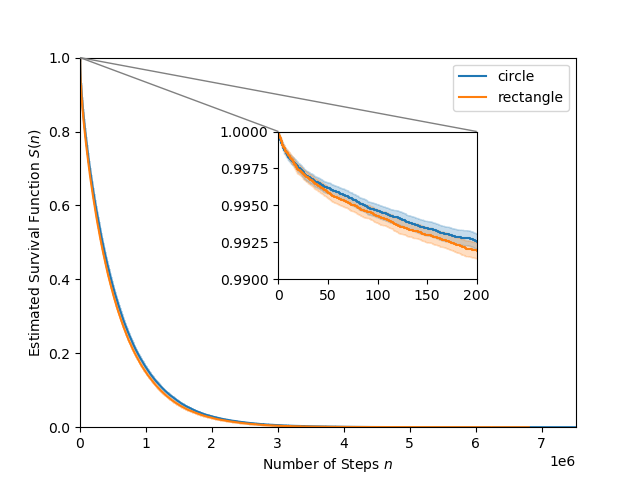
\includegraphics[width=\textwidth]{circle_rect_steps_sf.png}
     \label{fig:sf_simple_shape_steps}
     \caption{In the inset, the decay rate of the survival function for the rectangle is slightly larger than for the circle, which coincides with the theoretical result.}
   \end{figure}

  The differences between survival functions for the circle and
  rectangle are not visible. Moreover, the approximate $95\%$
  confidence intervals of the survival functions overlap. In this
  case, non-parametric statistical tests can be used to compare entire
  survival distributions and assess their dissimilarities. The logrank
  test has maximum power if the proportional hazards assumption is
  satisfied. 

   \begin{figure}
     \centering
     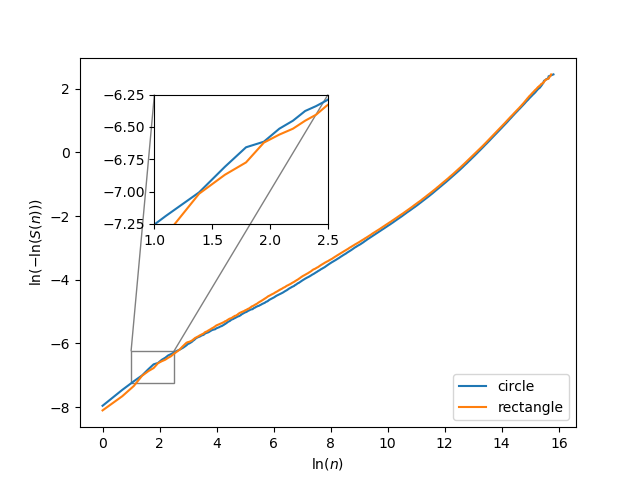
\includegraphics[width=\textwidth]{circle_rect_steps_ph.png}
     \label{fig:ph_test_simple_shapes}
     \caption{It is a graphical method for checking proportionality by looking for parallelism. As shown in the inset plot, two curves cross at some points and their shapes vary over time. Moreover, $p < 0.05$ in the non-proportional test. Thus, the survival functions for circle and rectangle do not satisfy the proportional hazard assumption.}
   \end{figure}


   \begin{table}
     \centering
     \begin{tabular}{lrr}
        \toprule
         {} &  test\_statistic &             p \\
         \midrule
         Logrank & 137.23 & 0.0 \\
         \midrule
         Tarone-Ware & 134.31 & 0.0 \\
         \midrule
         Gehan-Breslow & 123.83 & 0.0 \\
         \midrule
         Fleming-Harrington & 123.83 & 0.0 \\
         \bottomrule
     \end{tabular}
     \caption{Survival functions for circle and rectangle are statistically different since p values equal zeros.}
     \label{tab:test_simple_shape_steps}
   \end{table}



\subsection{Conclusion}


Although the proportional hazard assumption test is failed as shown in
Fig.~\ref{fig:ph_test_simple_shapes}, the weighted logrank tests
indicate that the null hypothesis should be rejected. In conclusion,
LRWs is an alternative tool to quantify and distinguish the geometries
in the $2-$ dimensional image without measuring the predefined shape
descriptors.
  
